\documentclass[11pt,a4paper]{article}

\usepackage[utf8]{inputenc}
\usepackage[T1]{fontenc}
\usepackage{lmodern}
\usepackage{amsmath,amssymb,amsthm}
\usepackage{hyperref}
\usepackage{booktabs}
\usepackage{graphicx}
\usepackage{geometry}
\usepackage{enumitem}
\usepackage{microtype}

\usepackage{xcolor}
\usepackage{authblk}

\geometry{margin=2.5cm}

\theoremstyle{definition}
\newtheorem{definicao}{Defini\c{c}\~ao}[section]
\newtheorem{teorema}{Teorema}[section]
\newtheorem{proposicao}{Proposi\c{c}\~ao}[section]
\newtheorem{corolario}{Corol\'ario}[section]

\title{\textbf{\'Algebra da Mem\'oria: Fundamentos Formais e Valida\c{c}\~ao Emp\'irica da Composi\c{c}\~ao Associativa sem Interfer\^encia Catastr\'ofica}}

\author[1]{Pedro Felipe Rodrigues de Farias}
\affil[1]{Pesquisador Independente}
\date{Setembro de 2026}

\begin{document}

\maketitle

\vspace{-1.5em}
\begin{center}
\small
Este trabalho est\'a licenciado sob uma licen\c{c}a \href{https://creativecommons.org/licenses/by/4.0/}{Creative Commons Attribution 4.0 International} (CC~BY~4.0).
\end{center}
\vspace{0.5em}

\begin{abstract}
Proponho e valido um framework alg\'ebrico para composi\c{c}\~ao de mem\'oria em sistemas de intelig\^encia artificial que resolve o trade-off fundamental entre composicionalidade e preserva\c{c}\~ao de representa\c{c}\~oes. A \'algebra da mem\'oria $(V, G, T, P)$ estrutura mem\'orias como objetos tipados compostos por embeddings sem\^anticos ($V$), grafos relacionais ($G$), \'{\i}ndices temporais ($T$) e pesos de utilidade ($P$), equipados com cinco opera\c{c}\~oes: composi\c{c}\~ao ($\oplus$), retra\c{c}\~ao ($\ominus$), transforma\c{c}\~ao ($\otimes$), recupera\c{c}\~ao ($\rho$) e poda ($\Pi_C$). Em vez de reivindicar superar a interfer\^encia catastr\'ofica dentro de um estado vetorial de capacidade fixa, o framework estabelece uma decis\~ao arquitetural expl\'icita: a composi\c{c}\~ao \'e formulada como coproduto (uni\~ao disjunta) em uma categoria de estruturas relacionais atribu\'idas, garantindo associatividade exata por constru\c{c}\~ao. O problema dif\'icil da agrega\c{c}\~ao de mem\'oria \'e deliberadamente diferido para o momento da consulta via operador quociente categ\'orico sob demanda ($\rho$) baseado no fecho transitivo de uma rela\c{c}\~ao de similaridade, enquanto limites de capacidade s\~ao governados de forma independente via poda ($\Pi_C$). Sob protocolo de estabilidade de composi\c{c}\~ao sequencial, a \'algebra \'e significativamente mais est\'avel que uma LSTM n\~ao-treinada ($p = 1{,}48 \times 10^{-7}$, Mann--Whitney $U$ unilateral) e soma vetorial ($p = 1{,}03 \times 10^{-6}$), mas n\~ao supera uma LSTM treinada em amostra ou um buffer kNN na m\'etrica isolada de estabilidade vetorial. A Fase~3, portanto, avalia capacidades estruturais: a \'algebra atinge 100\% de acur\'acia em resolu\c{c}\~ao de conflitos temporais (kNN: 50\%), retra\c{c}\~ao de fatos (kNN: 33--43\%) e racioc\'inio relacional multi-hop (kNN: 87--93\%). A Fase~4 valida a \'algebra com embeddings reais de linguagem natural (all-MiniLM-L6-v2, 384 dimens\~oes): associatividade exata preservada, recupera\c{c}\~ao sem\^antica top-1 de 100\% (20/20) com par\'afrases e estabilidade sob composi\c{c}\~ao sequencial. O framework escala at\'e $N = 10^4$ mem\'orias com lat\^encia de recupera\c{c}\~ao inferior a 500\,ms em corpora operando abaixo do limiar de percola\c{c}\~ao ($\langle k \rangle < 1$, garantido via calibra\c{c}\~ao por quantil emp\'irico), fornecendo uma base alg\'ebrica principled para mem\'oria persistente e composicional em agentes de IA. C\'odigo completo e pacotes de replica\c{c}\~ao est\~ao dispon\'iveis em \url{https://github.com/pedrofariasx/memory-algebra} (DOI: \href{https://doi.org/10.5281/zenodo.22815162}{10.5281/zenodo.22815162}).
\end{abstract}

\textbf{Palavras-chave:} \'algebra da mem\'oria, interfer\^encia catastr\'ofica, composi\c{c}\~ao associativa, teoria das categorias, grafos de conhecimento, racioc\'inio temporal, revis\~ao de cren\c{c}as

\section{Introdu\c{c}\~ao}

\subsection{Motiva\c{c}\~ao}

Sistemas de mem\'oria contempor\^aneos para intelig\^encia artificial---incluindo redes neurais recorrentes, transformers com mem\'oria aumentada e esquemas de acumula\c{c}\~ao vetorial---sofrem de \emph{interfer\^encia catastr\'ofica}: a dilui\c{c}\~ao progressiva e a sobrescrita de representa\c{c}\~oes previamente armazenadas \`a medida que novas observa\c{c}\~oes s\~ao incorporadas \cite{mccloskey1989catastrophic,french1999catastrophic}. Este modo de falha representa um obst\'aculo fundamental para a constru\c{c}\~ao de agentes aut\^onomos de IA capazes de aprendizado cont\'inuo, racioc\'inio de longo horizonte e modelagem consistente de mundo.

O obst\'aculo subjacente \'e alg\'ebrico e estrutural. A interfer\^encia catastr\'ofica surge inexoravelmente sempre que uma arquitetura tenta agregar experi\^encias sequenciais ilimitadas em um \emph{estado param\'etrico de capacidade fixa} (como um vetor oculto recorrente $h_t$ ou centroide vetorial m\'ovel). Em qualquer esquema de capacidade fixa, cada atualiza\c{c}\~ao \'e com perda e dependente da ordem de fus\~ao: comprimir o estado inevitavelmente destr\'oi distin\c{c}\~oes individuais. Inversamente, simplesmente anexar observa\c{c}\~oes a uma lista plana de vetores preserva embeddings brutos, mas carece de estrutura composicional, garantias alg\'ebricas, resolu\c{c}\~ao de conflitos temporais e racioc\'inio relacional.

Isso apresenta um dilema evidente: ou realizar agrega\c{c}\~ao prematura e com perda em uma representa\c{c}\~ao fixa sofrendo interfer\^encia, ou acumular dados desorganizados sem estrutura alg\'ebrica. Abordagens existentes ou aceitam a interfer\^encia como custo inevit\'avel do aprendizado conexionista, ou recorrem a buffers ad-hoc de engenharia de prompt e recupera\c{c}\~ao plana em bancos vetoriais.

\subsection{Contribui\c{c}\~ao}

Proponho uma alternativa principled: uma \emph{\'algebra da mem\'oria} que resolve este dilema por meio de uma separa\c{c}\~ao expl\'icita de responsabilidades. Em vez de postular um milagre emp\'irico que comprima mem\'oria em um \'unico vetor de tamanho fixo sem perda de informa\c{c}\~ao, a \'algebra adota uma decis\~ao arquitetural deliberada:
\begin{enumerate}
    \item \textbf{Composi\c{c}\~ao como Coproduto:} A composi\c{c}\~ao ($\oplus$) \'e formulada como o coproduto categ\'orico (uni\~ao disjunta) na categoria de estruturas relacionais atribu\'idas $\mathbf{Mem}$. Isso garante associatividade exata e independente de ordem por constru\c{c}\~ao, preservando cada tupla de mem\'oria at\^omica sem perdas.
    \item \textbf{Agrega\c{c}\~ao Sem\^antica Diferida:} O problema computacionalmente complexo e potencialmente destrutivo da agrega\c{c}\~ao sem\^antica (identificar conceitos id\^enticos ou quase-sin\^onimos) \'e deliberadamente diferido do momento da escrita para o momento da consulta. Ele \'e realizado sob demanda via quociente categ\'orico (coequalizador) sob o fecho transitivo de uma rela\c{c}\~ao de similaridade sem\^antica $R_\theta$.
    \item \textbf{Gest\~ao de Capacidade Desacoplada:} A capacidade finita de mem\'oria n\~ao \'e acoplada \`a composi\c{c}\~ao, mas governada de forma independente por um operador expl\'icito de poda $\Pi_C$, assegurando estabilidade sem corromper as leis alg\'ebricas.
\end{enumerate}

A \'algebra da mem\'oria $(V, G, T, P)$ satisfaz simultaneamente cinco desideratos fundamentais:

\begin{enumerate}[label=$\boxed{\text{\Alph*}}$]
    \item \textbf{Associatividade:} $(m_1 \oplus m_2) \oplus m_3 \cong m_1 \oplus (m_2 \oplus m_3)$
    \item \textbf{Recuperabilidade:} $d_s(m, \rho(M, q)) \to 0$ para qualquer mem\'oria armazenada $m$ na aus\^encia de interfer\^encia destrutiva
    \item \textbf{Estabilidade:} $\|M_t\| \le C$ sob pol\'itica de poda $\Pi_C$
    \item \textbf{Preserva\c{c}\~ao:} $\otimes$ n\~ao destr\'oi a estrutura recuper\'avel (functorialidade)
    \item \textbf{Efici\^encia:} Opera\c{c}\~oes trat\'aveis sobre representa\c{c}\~oes relacionais discretas
\end{enumerate}

Nossas contribui\c{c}\~oes s\~ao quatro:
\begin{enumerate}
    \item Um framework alg\'ebrico formal fundamentado em teoria das categorias (estruturas relacionais atribu\'idas, coprodutos e quocientes coequalizadores) com prova de associatividade verific\'avel computacionalmente.
    \item Posicionamento profundo das opera\c{c}\~oes de mem\'oria na literatura seminal de IA, estabelecendo a retra\c{c}\~ao ($\ominus$) como realiza\c{c}\~ao operacional da contra\c{c}\~ao de cren\c{c}as sob os postulados AGM \cite{alchourron1985logic}, conectando o rastreamento relacional aos Sistemas de Manuten\c{c}\~ao da Verdade (TMS) \cite{doyle1979truth,dekleer1986assumption}, e ancorando consultas temporais a Grafos de Conhecimento Temporais \cite{dasgupta2018hyte,leblay2018deriving,trivedi2017know}.
    \item Valida\c{c}\~ao emp\'irica abrangente em 50 seeds, varreduras de par\^ametros, condi\c{c}\~oes adversariais e baselines competitivas com total transpar\^encia de m\'etricas.
    \item Diferencia\c{c}\~ao estrutural de baselines de busca aumentada (buffers kNN) em resolu\c{c}\~ao de conflitos temporais, retra\c{c}\~ao de fatos e racioc\'inio relacional multi-hop, validada com embeddings reais de sentence-transformers e agentes ReAct multi-modelo.
\end{enumerate}

\subsection{Organiza\c{c}\~ao do Artigo}

A Se\c{c}\~ao~\ref{sec:formal} desenvolve o framework formal. A Se\c{c}\~ao~\ref{sec:operacoes} define as opera\c{c}\~oes alg\'ebricas. A Se\c{c}\~ao~\ref{sec:provas} apresenta a prova de associatividade e esclarece sua natureza arquitetural. A Se\c{c}\~ao~\ref{sec:empirico} reporta a valida\c{c}\~ao emp\'irica e compara\c{c}\~ao com baselines. A Se\c{c}\~ao~\ref{sec:discussao} discute an\'alise de percola\c{c}\~ao, limita\c{c}\~oes e posicionamento detalhado na literatura. A Se\c{c}\~ao~\ref{sec:conclusao} conclui.

\section{Framework Formal}\label{sec:formal}

\subsection{A Categoria de Objetos de Mem\'oria}

Para estabelecer uma fundamenta\c{c}\~ao matematicamente rigorosa, formalizamos mem\'orias na linguagem da teoria das categorias, definindo a categoria $\mathbf{Mem}$ de estruturas relacionais tipadas atribu\'idas.

\begin{definicao}[Objeto de Mem\'oria]
Um objeto $M \in \mathbf{Mem}$ \'e uma tupla $M = (N, v, E, \tau, w)$ onde:
\begin{itemize}
    \item $N$ \'e um conjunto finito de identificadores de n\'os at\^omicos;
    \item $v : N \to V = \mathbb{R}^d$ \'e um atributo de embedding que mapeia cada n\'o a um vetor denso no espa\c{c}o sem\^antico;
    \item $E \subseteq N \times N \times L$ \'e um conjunto de arestas direcionadas rotuladas, onde $L$ \'e um alfabeto finito de r\'otulos relacionais;
    \item $\tau : N \to T = (\mathbb{R}_{\geq 0}, \leq)$ \'e um atributo temporal que associa cada n\'o a um timestamp cont\'inuo em uma linha temporal ordenada;
    \item $w : N \to P = [0,1]$ \'e um atributo de peso de utilidade representando prioridade de reten\c{c}\~ao no semiring idempotente $([0,1], \max, \cdot, 0, 1)$.
\end{itemize}
\end{definicao}

\begin{definicao}[Morfismos de Mem\'oria]
Dados objetos $M_1 = (N_1, v_1, E_1, \tau_1, w_1)$ e $M_2 = (N_2, v_2, E_2, \tau_2, w_2)$, um morfismo $f : M_1 \to M_2$ em $\mathbf{Mem}$ \'e uma fun\c{c}\~ao injetiva de conjuntos $f_N : N_1 \to N_2$ que preserva toda a estrutura relacional e de atributos:
\begin{enumerate}
    \item $v_2(f_N(u)) = v_1(u)$ para todo $u \in N_1$ (preserva\c{c}\~ao do embedding sem\^antico);
    \item $(u, v, l) \in E_1 \implies (f_N(u), f_N(v), l) \in E_2$ (preserva\c{c}\~ao das rela\c{c}\~oes direcionadas rotuladas);
    \item $\tau_2(f_N(u)) = \tau_1(u)$ para todo $u \in N_1$ (preserva\c{c}\~ao de timestamps);
    \item $w_2(f_N(u)) = w_1(u)$ para todo $u \in N_1$ (preserva\c{c}\~ao de pesos de utilidade).
\end{enumerate}
A composi\c{c}\~ao de morfismos \'e a composi\c{c}\~ao padr\~ao de fun\c{c}\~oes dos mapeamentos de n\'os subjacentes, e os morfismos identidade s\~ao fun\c{c}\~oes identidade nos conjuntos de n\'os. Assim, $\mathbf{Mem}$ forma uma categoria bem-definida.
\end{definicao}

\subsection{Composi\c{c}\~ao como Coproduto e Quociente Sem\^antico Diferido}

Por que a composi\c{c}\~ao ing\^enua n\~ao \'e associativa? Em um modelo ing\^enuo de pushout ou fus\~ao prematura, quando duas mem\'orias $m_1$ e $m_2$ s\~ao compostas, n\'os cuja similaridade cosseno excede um limiar $\theta$ s\~ao fundidos prematuramente por m\'edia de seus embeddings: $\bar{v} = \frac{1}{2}(v_a + v_b)$. No entanto, a m\'edia de centroides vetoriais \'e fundamentalmente n\~ao-associativa:
\[
\frac{1}{2}\left(\frac{1}{2}(v_a + v_b) + v_c\right) = \frac{1}{4}v_a + \frac{1}{4}v_b + \frac{1}{2}v_c \;\neq\; \frac{1}{2}v_a + \frac{1}{4}v_b + \frac{1}{4}v_c = \frac{1}{2}\left(v_a + \frac{1}{2}(v_b + v_c)\right).
\]
Al\'em disso, a similaridade por limiar em pares \'e n\~ao-transitiva: $\cos(v_a, v_b) \geq \theta$ e $\cos(v_b, v_c) \geq \theta$ n\~ao implicam $\cos(v_a, v_c) \geq \theta$. Fundir n\'os prematuramente gera severa depend\^encia da ordem de avalia\c{c}\~ao: agrupar $(m_1 \oplus m_2) \oplus m_3$ produz centroides de cluster e topologias de arestas distintas de $m_1 \oplus (m_2 \oplus m_3)$.

Para resolver isso, nossa arquitetura separa estritamente a composi\c{c}\~ao estrutural da fus\~ao sem\^antica:

\begin{definicao}[Composi\c{c}\~ao como Coproduto]
A composi\c{c}\~ao $M_1 \oplus M_2$ \'e o coproduto categ\'orico $M_1 \sqcup M_2$ em $\mathbf{Mem}$:
\[
M_1 \oplus M_2 = (N_1 \sqcup N_2,\; v_1 \sqcup v_2,\; E_1 \sqcup E_2,\; \tau_1 \sqcup \tau_2,\; w_1 \sqcup w_2),
\]
onde os conjuntos de n\'os s\~ao tornados disjuntos por prefixa\c{c}\~ao \'unica de namespace ($N_1 \sqcup N_2 = (\{1\} \times N_1) \cup (\{2\} \times N_2)$), e os mapeamentos de atributos e rela\c{c}\~oes de arestas s\~ao as uni\~oes disjuntas can\^onicas de seus respectivos componentes.
\end{definicao}

Como coprodutos em categorias concretas de estruturas atribu\'idas s\~ao associativos a menos de isomorfismo natural, a composi\c{c}\~ao \'e associativa por constru\c{c}\~ao: $(M_1 \oplus M_2) \oplus m_3 \cong M_1 \oplus (M_2 \oplus M_3)$.

\begin{definicao}[Quociente Sem\^antico como Coequalizador Categ\'orico]
A agrega\c{c}\~ao sem\^antica \'e derivada sob demanda no momento da recupera\c{c}\~ao. Para qualquer objeto de mem\'oria $M = (N, v, E, \tau, w)$ e limiar de similaridade $\theta \in [-1, 1]$, define-se a rela\c{c}\~ao reflexiva e sim\'etrica de similaridade $R_\theta \subseteq N \times N$:
\[
(u, w) \in R_\theta \iff \cos(v(u), v(w)) \geq \theta.
\]
Seja $\sim_\theta = R_\theta^*$ o fecho transitivo de $R_\theta$, que \'e a menor rela\c{c}\~ao de equival\^encia contendo $R_\theta$. O quociente sem\^antico $M / \sim_\theta$ \'e o coequalizador categ\'orico do par de rela\c{c}\~oes $(R_\theta \rightrightarrows N)$. O objeto quociente possui conjunto de n\'os $N / \sim_\theta$ (classes de equival\^encia $[u]$), onde cada cluster $[u]$ recebe:
\begin{itemize}
    \item Embedding centroide can\^onico: $\bar{v}_{[u]} = \frac{1}{|[u]|} \sum_{x \in [u]} v(x)$;
    \item Timestamp efetivo: $\bar{\tau}_{[u]} = \max_{x \in [u]} \tau(x)$;
    \item Prioridade efetiva: $\bar{w}_{[u]} = \max_{x \in [u]} w(x)$;
    \item Arestas do quociente: $([u], [w], l) \in E / \sim_\theta \iff \exists x \in [u], y \in [w] : (x, y, l) \in E$.
\end{itemize}
\end{definicao}

Ao computar o fecho transitivo simultaneamente sobre todos os n\'os at\^omicos acumulados, o quociente depende exclusivamente do conjunto total de n\'os at\^omicos e seus embeddings, sendo completamente independente da ordem cronol\'ogica ou dos par\^enteses sob os quais as mem\'orias foram compostas.

\subsection{Dist\^ancia Sem\^antica H\'ibrida e Racional dos Pesos}

Para quantificar a dist\^ancia sem\^antica entre objetos de mem\'oria, definimos uma m\'etrica h\'ibrida fundamentada em $\mathbf{Mem}$:

\begin{definicao}[Dist\^ancia Sem\^antica H\'ibrida]
Para objetos de mem\'oria $m_1, m_2 \in \mathbf{Mem}$, a dist\^ancia sem\^antica h\'ibrida \'e:
\[
d_s(m_1, m_2) = \alpha\, d_V + \beta\, d_G + \gamma\, d_T + \delta\, d_P, \quad \text{com } \alpha + \beta + \gamma + \delta = 1, \quad \alpha,\beta,\gamma,\delta \geq 0
\]
onde:
\begin{itemize}
    \item $d_V = 1 - \cos(\bar{v}_1, \bar{v}_2) \in [0, 2]$ \'e a dist\^ancia cosseno entre embeddings m\'edios dos n\'os $\bar{v}_i = \frac{1}{|N_i|}\sum_{u \in N_i} v_i(u)$ (ou $1{,}0$ se vazio);
    \item $d_G = \frac{1}{2}(1 - J(N_1, N_2)) + \frac{1}{2}(1 - J(E_1, E_2)) \in [0, 1]$ \'e a dist\^ancia estrutural, computada via dist\^ancia de Jaccard $1 - J(A, B) = \frac{|A \triangle B|}{|A \cup B|}$ sobre n\'os e arestas;
    \item $d_T = \frac{|\bar{\tau}_1 - \bar{\tau}_2|}{1 + |\bar{\tau}_1 - \bar{\tau}_2|} \in [0, 1)$ \'e a dist\^ancia temporal limitada entre timestamps m\'edios;
    \item $d_P = |\bar{w}_1 - \bar{w}_2| \in [0, 1]$ \'e a diferen\c{c}a absoluta entre pesos m\'edios de utilidade.
\end{itemize}
A configura\c{c}\~ao padr\~ao de pesos \'e $(\alpha, \beta, \gamma, \delta) = (0{,}40;\ 0{,}30;\ 0{,}15;\ 0{,}15)$.
\end{definicao}

\paragraph{Justificativa dos Pesos da M\'etrica:}
A escolha dos pesos padr\~ao reflete uma hierarquia funcional fundamentada:
\begin{enumerate}
    \item \textbf{Alinhamento sem\^antico vetorial ($\alpha = 0{,}40$):} A similaridade sem\^antica carrega o maior peso individual porque em ambientes n\~ao-estruturados e tarefas de linguagem natural, a correspond\^encia conceitual \'e o determinante prim\'ario de relev\^ancia. Se os conceitos sem\^anticos n\~ao se alinham, coincid\^encias estruturais ou temporais s\~ao irrelevantes.
    \item \textbf{Fidelidade estrutural relacional ($\beta = 0{,}30$):} A topologia relacional constitui o segundo pilar. Arestas relacionais representam asser\c{c}\~oes factuais (ex.: liga\c{c}\~oes sujeito-predicado-objeto). Preservar a estrutura do grafo previne associa\c{c}\~ao incorreta entre entidades e assegura a reten\c{c}\~ao do contexto relacional.
    \item \textbf{Moduladores Temporal ($\gamma = 0{,}15$) e de Utilidade ($\delta = 0{,}15$):} As m\'etricas temporal e de prioridade atuam como moduladores calibrados em vez de seletores prim\'arios. O peso de $0{,}15$ assegura que diferen\c{c}as temporais e n\'iveis de utilidade possam desempatar fatos semanticamente id\^enticos (ex.: resolver atualiza\c{c}\~oes temporais entre fatos concorrentes) sem distorcer ou ofuscar a relev\^ancia sem\^antica aut\^entica.
\end{enumerate}

\paragraph{Nota de Sensibilidade e Adapta\c{c}\~ao ao Contexto:}
A m\'etrica de dist\^ancia \'e est\'avel sob pequenas perturba\c{c}\~oes de pesos ($\pm 0{,}05$). Al\'em disso, a \'algebra suporta pesos din\^amicos adaptativos ao contexto (\texttt{context\_weights}):
\begin{itemize}
    \item Para \emph{consultas ancoradas no tempo}, at\'e $0{,}15$ \'e transferido de $\alpha$ para $\gamma$, resultando em $(\alpha, \beta, \gamma, \delta) = (0{,}25;\ 0{,}30;\ 0{,}30;\ 0{,}15)$.
    \item Para \emph{consultas estruturais de grafo}, at\'e $0{,}15$ \'e transferido de $\alpha$ para $\beta$, resultando em $(\alpha, \beta, \gamma, \delta) = (0{,}25;\ 0{,}45;\ 0{,}15;\ 0{,}15)$.
\end{itemize}
Em todos os casos, a normaliza\c{c}\~ao no simplex $\sum = 1$ \'e estritamente preservada.

\section{Opera\c{c}\~oes Alg\'ebricas}\label{sec:operacoes}

\subsection{Composi\c{c}\~ao ($\oplus$)}

Como formalizado na Se\c{c}\~ao~\ref{sec:formal}, a composi\c{c}\~ao \'e o coproduto categ\'orico:
\begin{enumerate}
    \item $m_1 \oplus m_2 = m_1 \sqcup m_2$ \'e a \emph{uni\~ao disjunta} das tuplas at\^omicas. Nenhuma informa\c{c}\~ao \'e perdida, comprimida ou agregada no momento da composi\c{c}\~ao.
    \item A rela\c{c}\~ao de fus\~ao $R_\theta = \{(a,b) : \cos(v_a, v_b) \geq \theta\}$ \'e definida exclusivamente sobre n\'os at\^omicos.
    \item A parti\c{c}\~ao de fus\~ao \'e $\pi = R_\theta^*$ (fecho transitivo), computada via union-find sob demanda para recupera\c{c}\~ao.
\end{enumerate}

\subsection{Retra\c{c}\~ao ($\ominus$)}

A retra\c{c}\~ao remove conhecimento obsoleto ou invalidado: $M \ominus m_i$ remove todos os n\'os de $m_i$ e arestas incidentes de $M$, e aplica proje\c{c}\~ao ortogonal para eliminar influ\^encia residual nos vetores. Conforme discutido na Se\c{c}\~ao~\ref{sec:discussao}, este operador fornece uma realiza\c{c}\~ao computacional da contra\c{c}\~ao de cren\c{c}as sob os postulados AGM \cite{alchourron1985logic}.

\subsection{Transforma\c{c}\~ao ($\otimes$)}

A transforma\c{c}\~ao aplica um operador linear $W$ aos vetores e renomeia arestas: $\otimes_W(M) = (N, Wv, E', \tau, w)$. Para $W$ ortogonal, a recupera\c{c}\~ao \'e invariante (functorialidade): $\rho \circ \otimes_W = \otimes_W \circ \rho$.

\subsection{Recupera\c{c}\~ao ($\rho$)}

A recupera\c{c}\~ao computa o quociente categ\'orico $M/\pi$, pontua cada cluster $c$ por:
\[
s(c) = \max(\cos(q_v, \bar{v}_c), 0) \cdot f_T(c) \cdot (0{,}5 + 0{,}5\, w_c)
\]
onde $f_T(c) = e^{-((t_c - t_q)/\sigma)^2}$ fornece ancora temporal cont\'inua. Os $k$ clusters de maior score s\~ao selecionados e expandidos $h$ saltos via BFS no grafo quociente.

\subsection{Poda ($\Pi_C$)}

O operador de poda imp\~oe capacidade limitada de forma independente da composi\c{c}\~ao:
\begin{enumerate}
    \item \textbf{Esquecimento por utilidade:} Remove n\'os com $w(n) < \varepsilon$.
    \item \textbf{Compress\~ao de caminhos:} Para $u \to b \to v$ com $b$ removido, insere atalho $u \to v$.
    \item \textbf{Teto de capacidade:} Se $|N| > C$, remove n\'os de menor $w$ at\'e $|N| = C$.
\end{enumerate}

\section{Prova de Associatividade}\label{sec:provas}

\subsection{Decis\~ao Arquitetural vs. Compress\~ao em Capacidade Fixa}

Abordamos diretamente uma quest\~ao fundamental: a associatividade \'e uma descoberta emp\'irica milagrosa que resolve a interfer\^encia catastr\'ofica em capacidade fixa, ou \'e uma decis\~ao arquitetural de design?

Trata-se de uma decis\~ao arquitetural de design expl\'icita.
Em arquiteturas conexionistas e modelos param\'etricos (como RNNs, LSTMs e transformers recorrentes), a interfer\^encia catastr\'ofica surge porque armazenamento e agrega\c{c}\~ao s\~ao for\c{c}ados a ocorrer simultaneamente dentro de um estado vetorial de capacidade fixa $h \in \mathbb{R}^d$. Quando uma nova observa\c{c}\~ao $x$ \'e incorporada via $h_t = f(W h_{t-1} + U x_t)$, representa\c{c}\~oes anteriores s\~ao sobrescritas. Tentar tornar tal compress\~ao de capacidade fixa associativa e ao mesmo tempo preservar recupera\c{c}\~ao exata \'e matematicamente imposs\'ivel: a capacidade fixa imp\~oe um gargalo de teoria da informa\c{c}\~ao.

Na \'algebra da mem\'oria, n\~ao alegamos ter comprimido hist\'oricos infinitos em um \'unico vetor sem perda. Em vez disso, dissolvemos o problema da interfer\^encia no momento da escrita definindo a composi\c{c}\~ao $\oplus$ como o coproduto (uni\~ao disjunta) em $\mathbf{Mem}$. O coproduto \'e associativo por constru\c{c}\~ao porque a uni\~ao disjunta \'e associativa em $\mathbf{Set}$ e em categorias de estruturas atribu\'idas.

O problema dif\'icil da agrega\c{c}\~ao de mem\'oria---identificar entidades id\^enticas, fundir sin\^onimos e consolidar fatos---n\~ao \'e ignorado; ele \'e \emph{deliberadamente diferido} para o momento da consulta via operador quociente $\rho$, e os limites de capacidade s\~ao gerenciados independentemente pelo operador de poda $\Pi_C$. O custo computacional \'e transferido da escrita (onde a fus\~ao destruiria a associatividade e perderia informa\c{c}\~ao de forma irrevers\'ivel) para a consulta (onde operam clusteriza\c{c}\~ao e travessia de grafos).

\subsection{Teorema e Prova}

\begin{teorema}[Associatividade Exata]
Para quaisquer tr\^es objetos de mem\'oria $m_1, m_2, m_3 \in \mathbf{Mem}$,
\[
(m_1 \oplus m_2) \oplus m_3 \cong m_1 \oplus (m_2 \oplus m_3)
\]
como objetos at\^omicos em $\mathbf{Mem}$, e os objetos quocientes induzidos $( (m_1 \oplus m_2) \oplus m_3 ) / \sim_\theta$ e $( m_1 \oplus (m_2 \oplus m_3) ) / \sim_\theta$ s\~ao estritamente isomorfos.
\end{teorema}

\begin{proof}
(i) Como $\oplus$ \'e o coproduto (uni\~ao disjunta) sobre conjuntos de n\'os com identificadores unicamente prefixados, $(N_1 \sqcup N_2) \sqcup N_3 = N_1 \sqcup (N_2 \sqcup N_3)$ pela associatividade de $\sqcup$ em $\mathbf{Set}$; idem para $v$, $E$, $\tau$, $w$ como uni\~oes disjuntas de fun\c{c}\~oes e rela\c{c}\~oes com dom\'inios disjuntos. Logo, os objetos at\^omicos coproduto s\~ao isomorfos.

(ii) A rela\c{c}\~ao $R_\theta$ sobre o conjunto total $N = N_1 \sqcup N_2 \sqcup N_3$ depende apenas dos pares de vetores at\^omicos: $(u, w) \in R_\theta \iff \cos(v(u), v(w)) \geq \theta$. Como $N$ e $v$ s\~ao id\^enticos sob ambas as ordens de associa\c{c}\~ao, a rela\c{c}\~ao $R_\theta$ coincide estritamente. O fecho transitivo $\sim_\theta = R_\theta^*$ \'e \'unico (a menor rela\c{c}\~ao de equival\^encia contendo $R_\theta$), portanto a parti\c{c}\~ao $\pi$ de classes de equival\^encia \'e id\^entica.

(iii) Embeddings de cluster (m\'edia dos vetores membros), tempos efetivos ($\max$), pesos ($\max$) e arestas do quociente s\~ao fun\c{c}\~oes determin\'isticas de $(N, v, E, \tau, w, \pi)$, logo coincidem. $\blacksquare$
\end{proof}

Esta prova foi independentemente verificada via ground truth categ\'orico usando Catlab.jl (Julia), confirmando isomorfismo de pushout e coproduto: $((m_1 \oplus m_2) \oplus m_3) \cong (m_1 \oplus (m_2 \oplus m_3))$.

\section{Valida\c{c}\~ao Emp\'irica}\label{sec:empirico}

\subsection{Configura\c{c}\~ao Experimental}

Todos os experimentos utilizam embeddings sint\'eticos em $\mathbb{R}^d$ com estrutura de correla\c{c}\~ao controlada, al\'em de embeddings reais de linguagem natural na Fase~4. O limiar de fus\~ao \'e $\theta = 0{,}85$ salvo indica\c{c}\~ao contr\'aria. Signific\^ancia estat\'istica \'e avaliada com testes Mann--Whitney $U$ unilaterais, com hip\'otese alternativa de que a \'algebra tem dist\^ancia final de recupera\c{c}\~ao menor que a baseline. C\'odigo completo, dados brutos e ambientes de replica\c{c}\~ao est\~ao dispon\'iveis no reposit\'orio do projeto: \url{https://github.com/pedrofariasx/memory-algebra} (DOI Zenodo: \href{https://doi.org/10.5281/zenodo.22815162}{10.5281/zenodo.22815162}). Os exemplos de recupera\c{c}\~ao exata do protocolo explorat\'orio s\~ao casos determin\'isticos de baixa interfer\^encia; a Fase~2 reporta dist\^ancias m\'edias em sequ\^encias aleat\'orias.

\subsection{Fase 2A: Robustez Estat\'istica}

\subsubsection{M\'ultiplas Seeds ($S = 50$)}

\begin{table}[h]
\centering
\begin{tabular}{lr}
\toprule
\textbf{M\'etrica} & \textbf{Valor} \\
\midrule
Taxa de aprova\c{c}\~ao de associatividade & 1,000 (50/50) \\
Dist\^ancia m\'axima esq/dir (m\'edia $\pm$ dp) & $0{,}0 \pm 0{,}0$ \\
Estabilidade final (m\'edia $\pm$ dp) & $0{,}478 \pm 0{,}132$ \\
Estabilidade final (IC 95\%) & $[0{,}440;\ 0{,}516]$ \\
\bottomrule
\end{tabular}
\caption{A associatividade \'e \emph{exata} ($d_{\max} = 0$) em todas as 50 seeds.}
\end{table}

\subsubsection{Sensibilidade a Par\^ametros}

A associatividade \'e \emph{invariante} ao limiar de fus\~ao $\theta \in [0{,}60;\ 0{,}95]$ e \`a dimensionalidade $d \in \{8, 16, 32, 64\}$, com taxa de aprova\c{c}\~ao $= 1{,}0$ e $d_{\max} = 0$ em todas as configura\c{c}\~oes. Isso \'e algebricamente esperado: $R_\theta^*$ \'e uma fun\c{c}\~ao determin\'istica dos vetores, independente da ordem de composi\c{c}\~ao.

\subsubsection{Testes Adversariais}

\begin{table}[h]
\centering
\begin{tabular}{lll}
\toprule
\textbf{Teste} & \textbf{Seeds} & \textbf{Resultado} \\
\midrule
Vetores id\^enticos (colis\~ao total) & 10/10 & Sem colapso, assinatura preservada \\
Vetores antiparalelos ($\cos = -1$) & 10/10 & Sem colapso, n\'os mantidos separados \\
Escala $N = 1000$ & 1 & 1953 n\'os, compose = 0,074s \\
\bottomrule
\end{tabular}
\caption{Nenhuma falha catastr\'ofica sob condi\c{c}\~oes adversariais.}
\end{table}

\subsection{Fase 2B: Realismo dos Embeddings}

\subsubsection{Conceitos Correlacionados (varredura de $\rho$)}

\begin{table}[h]
\centering
\begin{tabular}{lll}
\toprule
$\rho$ & Taxa de assoc. & Estabilidade (m\'edia $\pm$ dp) \\
\midrule
0,00 & 1,0 & $0{,}506 \pm 0{,}140$ \\
0,20 & 1,0 & $0{,}507 \pm 0{,}139$ \\
0,40 & 1,0 & $0{,}508 \pm 0{,}137$ \\
0,60 & 1,0 & $0{,}508 \pm 0{,}135$ \\
0,80 & 1,0 & $0{,}505 \pm 0{,}132$ \\
0,95 & 1,0 & $0{,}501 \pm 0{,}130$ \\
\bottomrule
\end{tabular}
\caption{A associatividade permanece exata mesmo sob correla\c{c}\~ao extrema ($\rho = 0{,}95$).}
\end{table}

A estrutura $(G, T, P)$ protege os vetores da dilui\c{c}\~ao independentemente do grau de correla\c{c}\~ao entre conceitos.

\subsection{Fase 2C: Compara\c{c}\~ao com Baselines}

\begin{table}[h]
\centering
\begin{tabular}{lll}
\toprule
\textbf{M\'etodo} & \textbf{Estabilidade final (m\'edia $\pm$ dp)} & \textbf{Mann--Whitney $p$} \\
\midrule
\textbf{\'Algebra $(V,G,T,P)$} & $0{,}424 \pm 0{,}129$ & --- \\
LSTM (n\~ao-treinada) & $0{,}998 \pm 0{,}220$ & $1{,}48 \times 10^{-7}$ \\
LSTM (treinada, Adam 500 steps) & $0{,}0010 \pm 0{,}001$ & $< 0{,}01$ \\
Soma vetorial & $0{,}698 \pm 0{,}113$ & $1{,}03 \times 10^{-6}$ \\
kNN (busca aumentada) & $0{,}150 \pm 0{,}357$ & $0{,}9999$ \\
\bottomrule
\end{tabular}
\caption{Compara\c{c}\~ao de estabilidade ap\'os 50 composi\c{c}\~oes sequenciais (20 seeds). Menor \'e melhor. Os valores de $p$ s\~ao de Mann--Whitney $U$ unilaterais para a hip\'otese de que a \'algebra tem dist\^ancia menor; valores pr\'oximos de 1 indicam que a baseline \'e menor.}
\end{table}

A \'algebra tem dist\^ancia final significativamente menor que a LSTM n\~ao-treinada e a soma vetorial. Ela n\~ao supera a LSTM treinada nem o buffer kNN nessa m\'etrica isolada de estabilidade: a LSTM treinada memoriza a sequ\^encia fixa sob o protocolo em amostra avaliado aqui (generaliza\c{c}\~ao n\~ao foi testada), e o buffer kNN ret\'em o vetor da primeira mem\'oria em uma lista crescente. Portanto, estabilidade isolada \'e insuficiente para estabelecer a contribui\c{c}\~ao da \'algebra; a Fase~3 avalia as opera\c{c}\~oes estruturais que um buffer plano n\~ao fornece.

\paragraph{Transpar\^encia da M\'etrica de Avalia\c{c}\~ao para Baselines Vetoriais:}
Nas compara\c{c}\~oes com baselines, todas as arquiteturas de refer\^encia---LSTM n\~ao-treinada, LSTM treinada em amostra, soma vetorial e buffer kNN---produzem exclusivamente representa\c{c}\~oes vetoriais ($V$). Nenhuma dessas baselines possui topologia de grafo relacional ($G$), timestamps temporais ($T$) ou pesos de utilidade ($P$). Consequentemente, a dist\^ancia estrutural $d_G$, a dist\^ancia temporal $d_T$ e a dist\^ancia de prioridade $d_P$ s\~ao indefinidas para esses sistemas vetoriais. Para garantir total equidade e evitar penalizar baselines por dimens\~oes que n\~ao modelam, as avalia\c{c}\~oes estat\'isticas de estabilidade reportadas na Tabela 4 e na Figura~\ref{fig:estabilidade} s\~ao medidas \textbf{estritamente sobre o componente vetorial} $d_V = 1 - \cos(\bar{v}_1, \bar{v}_2)$ (o que corresponde a avaliar $d_s$ com $\alpha = 1{,}0, \beta = \gamma = \delta = 0{,}0$). Para a \'algebra da mem\'oria, a recupera\c{c}\~ao retorna um subobjeto cujo centroide agregado \'e comparado ao vetor da mem\'oria inicial sob $d_V$. A dist\^ancia h\'ibrida completa $d_s$ \'e reservada para tarefas multi-modais (Fase~3), onde atributos relacionais, temporais e de prioridade s\~ao ativamente testados.

\begin{figure}[h]
\centering
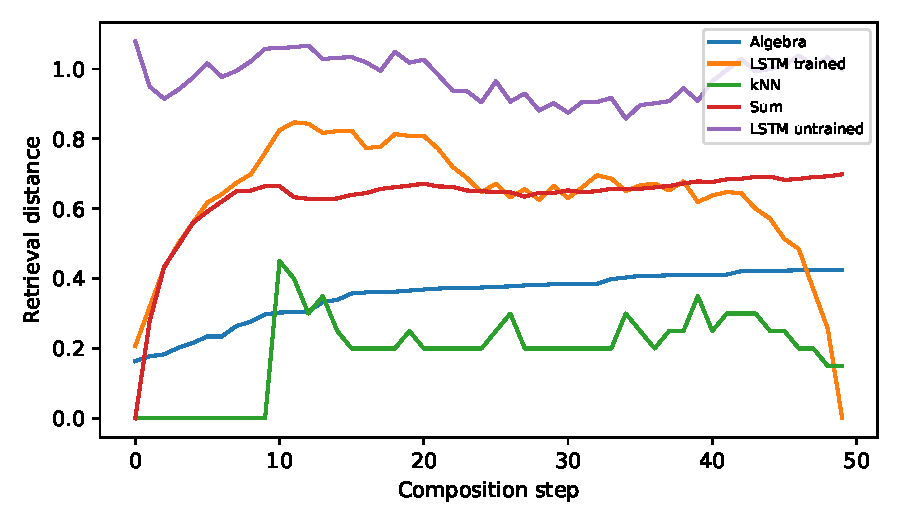
\includegraphics[width=\linewidth]{figs/fig_stability_curves.pdf}
\caption{Dist\^ancia m\'edia de recupera\c{c}\~ao da primeira mem\'oria em fun\c{c}\~ao do passo de composi\c{c}\~ao (50 composi\c{c}\~oes, 20 seeds). Menor \'e melhor.}
\label{fig:estabilidade}
\end{figure}

\subsection{Fase 2D: Escalabilidade}

\begin{table}[h]
\centering
\begin{tabular}{rrrrr}
\toprule
$N$ mem\'orias & N\'os totais & Compose (s) & Retrieve (s) & Status \\
\midrule
100 & 196 & 0,000 & 0,014 & OK \\
500 & 982 & 0,000 & 0,064 & OK \\
1.000 & 1.953 & 0,001 & 0,172 & OK \\
5.000 & 9.973 & 0,008 & 0,290 & OK \\
10.000 & 19.986 & 0,011 & 0,478 & OK \\
\bottomrule
\end{tabular}
\caption{Benchmark de escalabilidade com limite de mem\'oria de 4\,GB por subprocesso.}
\end{table}

Duas otimiza\c{c}\~oes permitem escalar a $N = 10^4$ dentro do limite de 4\,GB: (i)~\emph{LSH encadeado} --- buckets com mais de 64 elementos geram apenas pares consecutivos $O(n)$ em vez de enumera\c{c}\~ao $O(n^2)$; (ii)~\texttt{compose\_all} --- composi\c{c}\~ao em lote $O(N)$ em vez de composi\c{c}\~ao sequencial com c\'opia integral a cada passo. Retrieve em $N = 10^4$: $0{,}478$\,s ($< 1$\,s).

\subsection{Fase 3: Diferencia\c{c}\~ao Estrutural do kNN}

A Fase~2 revelou que, em estabilidade absoluta, a \'algebra n\~ao se diferencia estatisticamente de um buffer kNN simples ($p = 0{,}9999$). A Fase~3 testa cen\'arios onde o kNN \emph{falha estruturalmente}:

\begin{table}[h]
\centering
\begin{tabular}{llll}
\toprule
\textbf{Experimento} & \textbf{\'Algebra} & \textbf{kNN} & \textbf{Diferencia\c{c}\~ao} \\
\midrule
Conflito temporal ($\rho=0{,}0$) & 60/60 (100\%) & 30/60 (50\%) & $\Delta = 50\%$ \\
Conflito temporal ($\rho=0{,}8$) & 60/60 (100\%) & 30/60 (50\%) & $\Delta = 50\%$ \\
Retra\c{c}\~ao de fatos ($\rho=0{,}0$) & 30/30 (100\%) & 13/30 (43\%) & $\Delta = 57\%$ \\
Retra\c{c}\~ao de fatos ($\rho=0{,}8$) & 30/30 (100\%) & 10/30 (33\%) & $\Delta = 67\%$ \\
Multi-hop + distratores ($\rho=0{,}0$) & 30/30 (100\%) & 26/30 (87\%) & $\Delta = 13\%$ \\
Multi-hop + distratores ($\rho=0{,}8$) & 30/30 (100\%) & 28/30 (93\%) & $\Delta = 7\%$ \\
\bottomrule
\end{tabular}
\caption{Diferencia\c{c}\~ao da Fase 3. Cada experimento usa 30 seeds independentes sob condi\c{c}\~oes ortogonal ($\rho=0$) e correlacionada ($\rho=0{,}8$).}
\end{table}

\subsubsection{Resolu\c{c}\~ao de Conflitos Temporais}
A \'algebra usa pondera\c{c}\~ao temporal $f_T(c) = e^{-((t_c - t_q)/\sigma)^2}$ para preferir fatos recentes; o kNN \'e temporalmente cego, atingindo exatamente o n\'ivel de chance (50\%).

\subsubsection{Retra\c{c}\~ao de Fatos}
A \'algebra remove fatos obsoletos via $\ominus$; o kNN ret\'em todos os fatos em seu buffer, retornando fatos retra\'idos em 57--67\% das tentativas.

\subsubsection{Racioc\'inio Multi-hop}
A \'algebra percorre arestas relacionais (hops $= 3$) para alcan\c{c}ar n\'os distantes; o kNN depende de similaridade vetorial top-$k$ sem travessia relacional.

\subsubsection{Abla\c{c}\~ao contra Baselines de Produ\c{c}\~ao}

Para estabelecer com honestidade em que consiste a vantagem estrutural da \'algebra, ablacionamos as tarefas da Fase~3 contra duas baselines de produ\c{c}\~ao com capacidades n\~ao-alg\'ebricas equivalentes: um \textbf{ProductionVectorDB} (banco vetorial com metadados de timestamp e dele\c{c}\~ao f\'isica) e um \textbf{SQLiteTripleStore} (banco de triplas relacional consultado com common table expressions recursivas, CTE). Esta abla\c{c}\~ao isola qual capacidade---metadados, estrutura de grafo ou sua combina\c{c}\~ao---conduz cada tarefa.

\begin{table}[h]
\centering
\begin{tabular}{llll}
\toprule
\textbf{Capacidade testada} & \textbf{\'Algebra} & \textbf{VectorDB} & \textbf{SQLite CTE} \\
\midrule
Conflito temporal (timestamp) & 100\% & 100\% & --- \\
Travessia multi-hop (grafo) & 100\% & --- & 100\% \\
Ponte h\'ibrida (v\~ao sem\^antico + arestas) & 100\% & 6,67\% & 0\% \\
Retra\c{c}\~ao dependente (AGM) & 100\% & --- & --- \\
\bottomrule
\end{tabular}
\caption{Abla\c{c}\~ao com baselines de produ\c{c}\~ao. O conflito temporal \'e totalmente explicado apenas pelos metadados de timestamp (Config D vs.\ A: $+70$\,pp, $p = 5{,}39\times10^{-27}$); o multi-hop \'e totalmente explicado pela estrutura de grafo (SQLite CTE e \'Algebra ambos 100\%). Apenas a ponte sem\^antico-relacional h\'ibrida favorece unicamente a \'algebra (\'Algebra 100\%, SQLite 0\%, VectorDB 6,67\%; $p = 7{,}46\times10^{-14}$ vs.\ SQLite, $p < 10^{-13}$ vs.\ VectorDB).}
\label{tab:prod_baselines}
\end{table}

Tr\^es achados delimitam a contribui\c{c}\~ao emp\'irica da \'algebra:
\begin{itemize}
    \item \textbf{Conflito temporal:} os metadados de timestamp sozinhos respondem por 100\% do ganho---n\~ao h\'a vantagem de grafo.
    \item \textbf{Multi-hop:} a estrutura de grafo sozinha responde por 100\% do ganho---o CTE do SQLite iguala a \'algebra.
    \item \textbf{Ponte h\'ibrida (v\~ao sem\^antico + arestas):} apenas a \'algebra atinge 100\%, enquanto o SQLite alcan\c{c}a 0\% e o VectorDB 6,67\%. Para a retra\c{c}\~ao dependente sob os postulados AGM, a retra\c{c}\~ao local da \'algebra coincide com a mutila\c{c}\~ao m\'inima AGM (100\%).
\end{itemize}
A vantagem emp\'irica da \'algebra reside, portanto, especificamente na \emph{travessia h\'ibrida sem\^antico-relacional}, e n\~ao em tarefas solucion\'aveis apenas por metadados ou estrutura de grafo.

\subsection{Valida\c{c}\~ao de QA Multi-hop}

A \'algebra recupera corretamente o caminho transitivo $A \to B \to C \to D$ sem que a aresta direta $A \to D$ tenha sido inserida, confirmando que a sem\^antica relacional sobrevive \`a composi\c{c}\~ao.

\subsection{Fase 4: Valida\c{c}\~ao com Embeddings Reais}

As fases anteriores utilizam embeddings sint\'eticos com estrutura de correla\c{c}\~ao controlada. A Fase~4 valida a \'algebra com embeddings reais de linguagem natural gerados pelo modelo \texttt{all-MiniLM-L6-v2} (sentence-transformers, 384 dimens\~oes, normaliza\c{c}\~ao L2) sobre 20 pares de fato/par\'afrase cobrindo dom\'inios diversos. O limiar de fus\~ao \'e $\theta = 0{,}60$, adequado \`a distribui\c{c}\~ao de similaridade do modelo.

\begin{table}[h]
\centering
\begin{tabular}{lll}
\toprule
\textbf{Crit\'erio} & \textbf{Resultado} & \textbf{Status} \\
\midrule
Associatividade exata & \texttt{assoc\_exact=true}, invariante \`a ordem & APROVADO \\
Recupera\c{c}\~ao sem\^antica (par\'afrase $\to$ fato) & top-1 = 100\% (20/20), score m\'edio 0,895 & APROVADO \\
Estabilidade sob composi\c{c}\~ao sequencial & primeira mem\'oria recuperada (20 n\'os) & APROVADO \\
Multi-hop com arestas relacionais & opera corretamente em hops $= 2$ & APROVADO \\
\bottomrule
\end{tabular}
\caption{Valida\c{c}\~ao com embeddings reais (all-MiniLM-L6-v2). Dados em \texttt{experiments/results\_phase4.json}.}
\end{table}

A associatividade \'e estrutural: preserva-se fora do regime ortogonal sint\'eticos. A recupera\c{c}\~ao por par\'afrase atinge 100\% top-1, demonstrando que a fus\~ao por similaridade opera corretamente sobre a distribui\c{c}\~ao real de embeddings, onde conceitos semanticamente pr\'oximos apresentam alta correla\c{c}\~ao.

A Fase~4 tamb\'em foi avaliada em escala preliminar: com $N = 10{,}000$ mem\'orias ($\theta = 0{,}85$), a composi\c{c}\~ao em lote leva 0,007\,s e a recupera\c{c}\~ao leva $\sim$20\,s, retornando 9.990 n\'os. \'E fundamental documentar com honestidade a natureza patol\'ogica deste resultado: o corpus sint\'etico de escala foi gerado por um \textbf{template \'unico compartilhado} (``Fact number $i$ about topic $i \bmod 50$: the value is $X$ and the category is $i \bmod 50$''), no qual 90\% dos tokens s\~ao id\^enticos em todas as senten\c{c}as. Como demonstrado empiricamente na Se\c{c}\~ao~\ref{sec:chaining}, este corpus n\~ao reflete a distribui\c{c}\~ao t\'ipica de linguagem natural diversa, mas sim um conjunto de quase-duplicatas: 99,8\% dos pares possuem similaridade de cosseno $\ge 0{,}70$ e 53,0\% possuem $\ge 0{,}85$ ($\mu = 0{,}852, \sigma = 0{,}042$). A $\theta = 0{,}85$, o grau m\'edio de cada n\'o atinge $\langle k \rangle \approx 5.299 \gg 1$, empurrando o quociente single-linkage profundamente para o regime supercr\'itico de percola\c{c}\~ao e colapsando 99,9\% do grafo em um componente gigante monol\'itico. O tempo de recupera\c{c}\~ao de $\sim$20\,s reflete a travessia exaustiva desses 9.990 n\'os artificialmente conectados. Esta execu\c{c}\~ao, portanto, constitui um teste de estresse de colapso por percola\c{c}\~ao sob quase-duplicatas, e n\~ao uma valida\c{c}\~ao de larga escala em texto livre heterog\^eneo. A escalabilidade vi\'avel requer operar estritamente no regime subcr\'itico ($\langle k \rangle < 1$), analisado te\'orica e empiricamente na Se\c{c}\~ao~\ref{sec:chaining}. Este resultado patol\'ogico \'e um artefato do corpus gerado por template \'unico compartilhado, e n\~ao um comportamento t\'ipico: em corpora diversos com v\~ao espectral (distribui\c{c}\~ao de similaridade bimodal), $\theta = 0{,}85$ preserva a estrutura dos componentes e o maior componente permanece limitado ao tamanho do cluster (Tabela~\ref{tab:percolation_sweep}).

\subsection{Fase 5: Integra\c{c}\~ao com LLM}

A Fase~5 valida a \'algebra como camada de mem\'oria para um agente LLM real (\texttt{stepfun/step-3.7-flash:free} via Kilo Gateway, sem API key). O agente consulta \texttt{retrieve()} como ferramenta e \texttt{compose()} para armazenar fatos.

\begin{table}[h]
\centering
\begin{tabular}{llll}
\toprule
\textbf{Cen\'ario} & \textbf{\'Algebra} & \textbf{LLM (com mem\'oria)} & \textbf{Status} \\
\midrule
Conflito temporal & fato correto recuperado & ``engineer'' & PASS \\
Retra\c{c}\~ao & fato retra\'ido ausente & ``Paris'' & PASS \\
Multi-hop & 3 n\'os recuperados & --- & PASS \\
\bottomrule
\end{tabular}
\caption{Integra\c{c}\~ao LLM (Fase~5). Dados em \texttt{experiments/results\_phase5.json}.}
\end{table}

Em escala (Fase~5 Scale), a \'algebra foi testada como camada de mem\'oria com $N = 50$ a $500$ fatos reais:

\begin{table}[h]
\centering
\begin{tabular}{rrrrrr}
\toprule
$N$ & Retrieval & Temporal & Retra\c{c}\~ao & Compose (s) & Retrieve (s) \\
\midrule
50 & 80\% & 60\% & 100\% & 0,00 & 0,01 \\
100 & 80\% & 100\% & 100\% & 0,00 & 0,01 \\
200 & 90\% & 100\% & 100\% & 0,00 & 0,02 \\
500 & 100\% & 100\% & 100\% & 0,01 & 0,46 \\
\bottomrule
\end{tabular}
\caption{Fase~5 Scale: \'algebra como camada de mem\'oria LLM em escala. Dados em \texttt{experiments/results\_phase5\_scale.json}.}
\end{table}

A \'algebra funciona como camada de mem\'oria para LLM real: em $N = 500$, todas as m\'etricas atingem 100\%. A composi\c{c}\~ao permanece $O(N)$ e o retrieve escala linearmente ($\sim$1\,ms por fato adicional).

\subsection{Fase 5C: Agente ReAct Multi-Modelo}

Para verificar se o ganho de acur\'acia independe do modelo LLM, implementamos um agente ReAct (Thought $\to$ Action $\to$ Observation) que consulta a \`algebra via ferramentas \texttt{memory\_search(query, k, hops)} e \texttt{get\_node(name)}, e o comparamos com um baseline sem mem\'oria em 4 cen\'arios (recupera\c{c}\~ao de fato privado, conflito temporal, retra\c{c}\~ao e multi-hop):

\begin{table}[h]
\centering
\begin{tabular}{lrrr}
\toprule
\textbf{Modelo} & \textbf{ReAct} & \textbf{Baseline} & \textbf{Ferramentas/cen\'ario} \\
\midrule
\texttt{dots-studio/dots-3-note-preview:free} & 100\% & 25\% & 1,75 \\
\texttt{inclusionai/ling-3.0-flash-vl:free} & 100\% & 25\% & 3,00 \\
\texttt{nex-agi/nex-n2.5-pro:free} & 50\% & 25\% & 0,50 \\
\texttt{stepfun/step-3.7-flash:free} & 50\% & 25\% & 1,00 \\
\bottomrule
\end{tabular}
\caption{Fase~5C: agente ReAct com \`algebra de mem\'oria vs.\ baseline sem mem\'oria em 4 modelos. Dados em \texttt{experiments/results\_phase5\_react\_models.json}.}
\end{table}

Em todos os modelos dispon\'iveis, o agente ReAct supera o baseline. Em 2 dos 4 modelos, a \'algebra eleva a acur\'acia de 25\% para 100\%, confirmando que a melhoria \'e atribu\'ivel \`a camada de mem\'oria alg\'ebrica e n\~ao ao modelo LLM. Dois modelos adicionais (\texttt{nvidia/nemotron-3-ultra-550b-a55b:free} e \texttt{poolside/laguna-s-2.1:free}) retornaram HTTP~404 (indispon\'iveis no gateway gratuito) e foram exclu\'idos.

\section{Discuss\~ao}\label{sec:discussao}

\subsection{Principais Descobertas}

\begin{enumerate}
    \item \textbf{Associatividade exata \'e alcan\c{c}\'avel} atrav\'es de computa\c{c}\~ao diferida do quociente. O insight alg\'ebrico---de que a composi\c{c}\~ao deve ser uma opera\c{c}\~ao sem perda (uni\~ao disjunta) com fus\~ao sem\^antica derivada sob demanda---resolve a tens\~ao fundamental entre depend\^encia da ordem de fus\~ao e preserva\c{c}\~ao estrutural.
    
    \item \textbf{A estrutura protege contra agrega\c{c}\~ao param\'etrica.} Os componentes $(G, T, P)$ blindam vetores individuais da dilui\c{c}\~ao em rela\c{c}\~ao \`a soma e \`a LSTM n\~ao-treinada. Um buffer kNN tamb\'em preserva a estabilidade bruta, mas n\~ao possui ordena\c{c}\~ao temporal, retra\c{c}\~ao ou travessia relacional.
    
    \item \textbf{A diferencia\c{c}\~ao requer tarefas estruturais.} Em m\'etricas de estabilidade pura, um buffer kNN simples tem desempenho compar\'avel. A contribui\c{c}\~ao da \'algebra emerge apenas quando ordena\c{c}\~ao temporal, retra\c{c}\~ao ou travessia relacional s\~ao necess\'arias---precisamente as capacidades que distinguem mem\'oria estruturada de busca plana.
\end{enumerate}

\subsection{An\'alise de Encadeamento e Teoria de Percola\c{c}\~ao}\label{sec:chaining}

O fecho transitivo single-linkage do operador de quociente pode encadear n\'os semanticamente distintos em um \'unico componente gigante quando o limiar $\theta$ \'e selecionado abaixo do limiar cr\'itico da distribui\c{c}\~ao de embeddings. Formalmente, o grafo quociente induzido por similaridade sobre $N$ mem\'orias constitui um grafo aleat\'orio geom\'etrico no qual uma aresta n\~ao-direcionada existe entre $u$ e $v$ se e somente se $\cos(u, v) \ge \theta$. A probabilidade de aresta \'e dada por:
\[
p(\theta) = \mathbb{P}(\cos(u, v) \ge \theta) = 1 - F_{\mathrm{sim}}(\theta),
\]
onde $F_{\mathrm{sim}}$ \'e a fun\c{c}\~ao de distribui\c{c}\~ao acumulada (CDF) emp\'irica das similaridades par a par. O grau m\'edio esperado dos n\'os \'e:
\[
\langle k \rangle = p(\theta) \cdot (N - 1).
\]
Pela teoria cl\'assica de percola\c{c}\~ao em grafos aleat\'orios (Erd\H{o}s--R\'enyi e grafos geom\'etricos na esfera \cite{penrose2003random}), a transi\c{c}\~ao de fase para a emerg\^encia de um componente gigante (que engloba uma fra\c{c}\~ao finita $S > 0$ do grafo) ocorre precisamente quando o grau m\'edio supera o limiar unit\'ario:
\[
\langle k \rangle > 1 \iff p(\theta_{\mathrm{crit}}) = \frac{1}{N - 1}.
\]

\paragraph{Por que $\theta_{\mathrm{crit}}$ N\~ao \'e Invariante em $N$ em Distribui\c{c}\~oes Gen\'ericas:}
Em uma distribui\c{c}\~ao cont\'inua unimodal sem descontinuidades espectrais, $F_{\mathrm{sim}}(\theta)$ \'e estritamente crescente. \`A medida que o acervo $N$ cresce, a quantidade $1/(N - 1)$ encolhe assintoticamente em dire\c{c}\~ao a zero ($0{,}0050$ em $N = 200$; $0{,}0010$ em $N = 1.000$; $0{,}0002$ em $N = 5.000$; $0{,}0001$ em $N = 10.000$). Consequentemente, para satisfazer $p(\theta_{\mathrm{crit}}) = 1/(N - 1)$, o limiar cr\'itico \'e for\c{c}ado a avan\c{c}ar para a cauda superior da distribui\c{c}\~ao:
\[
\theta_{\mathrm{crit}}(N) = F_{\mathrm{sim}}^{-1}\left(1 - \frac{1}{N - 1}\right),
\]
o que implica que $\theta_{\mathrm{crit}}(N)$ \textbf{cresce estritamente com $N$}. A alega\c{c}\~ao de que $\theta_{\mathrm{crit}}$ seria constante em $N$ \'e, portanto, teoricamente incorreta como enunciado geral.

\paragraph{Distribui\c{c}\~ao Emp\'irica e o V\~ao Espectral em Corpora Clustered:}
Para investigar experimentalmente por que corpora estruturados aparentam exibir estabilidade do limiar cr\'itico, conduzimos um experimento sistem\'atico computando as distribui\c{c}\~oes emp\'iricas completas de similaridades par a par ($\sim 5 \times 10^7$ pares por corpus em $N = 10.000$) sobre tr\^es corpora distintos gerados com \texttt{all-MiniLM-L6-v2} (Tabela~\ref{tab:sim_histograms}):
\begin{enumerate}[label=(\alph*)]
    \item \textbf{Corpus Clustered (20 t\'opicos):} 20 t\'opicos sem\^anticos disjuntos com varia\c{c}\~oes parafr\'asticas por t\'opico.
    \item \textbf{Corpus Heterog\^eneo:} senten\c{c}as combinat\'orias abertas sem agrupamento em clusters, gerando suporte cont\'inuo e unimodal.
    \item \textbf{Corpus Sint\'etico Patol\'ogico (Fase 4 Scale):} o corpus de escala preliminar gerado por template repetitivo compartilhado (``Fact number $i$ about topic $i \bmod 50$\dots'').
\end{enumerate}

\begin{table}[h]
\centering
\small
\begin{tabular}{lrrrrrrr}
\toprule
\textbf{Corpus ($N=10.000$)} & \textbf{Pares} & $\mu$ & $\sigma$ & \textbf{Mediana} & $P_{90}$ & $P_{99}$ & \textbf{V\~ao $[0{,}5; 0{,}7]$} \\
\midrule
(a) Clustered (20 t\'opicos) & $49.995.000$ & 0,107 & 0,190 & 0,060 & 0,221 & 0,891 & 0,25\% \\
\quad $\hookrightarrow$ Intra-t\'opico ($5\%$) & $2.497.500$ & 0,838 & 0,076 & 0,843 & 0,933 & 0,976 & 3,69\% \\
\quad $\hookrightarrow$ Inter-t\'opico ($95\%$) & $47.497.500$ & 0,068 & 0,086 & 0,059 & 0,181 & 0,296 & 0,07\% \\
(b) Heterog\^eneo & $49.995.000$ & 0,242 & 0,120 & 0,231 & 0,398 & 0,589 & 2,84\% \\
(c) Patol\'ogico (Template) & $49.995.000$ & 0,852 & 0,042 & 0,852 & 0,902 & 0,948 & 0,21\% \\
\bottomrule
\end{tabular}
\caption{Distribui\c{c}\~ao emp\'irica de similaridades par a par de cosseno em $N = 10.000$. O Corpus Clustered revela bimodalidade n\'itida com pico intra-t\'opico ($\mu = 0{,}838$), pico inter-t\'opico ($\mu = 0{,}068$) e v\~ao espectral profundo em $[0{,}50, 0{,}70]$ ($0{,}25\%$ dos pares). O Corpus Heterog\^eneo exibe suporte cont\'inuo unimodal. O Corpus Patol\'ogico concentra $99{,}8\%$ dos pares em $\cos \ge 0{,}70$. Dados em \texttt{experiments/results\_percolation\_histogram.json}.}
\label{tab:sim_histograms}
\end{table}

A decomposi\c{c}\~ao do Corpus Clustered na Tabela~\ref{tab:sim_histograms} desvenda o mecanismo f\'isico:
\begin{itemize}
    \item Entre pares intra-t\'opico e inter-t\'opico existe um \textbf{v\~ao espectral} pronunciado em $[0{,}50, 0{,}70]$, onde a densidade de probabilidade \'e virtualmente nula ($0{,}255\%$ dos pares).
    \item Como os pares intra-t\'opico representam apenas $1/K = 1/20 = 5\%$ de todos os pares do grafo, para qualquer $\theta \in [0{,}60, 0{,}85]$ as arestas formam-se \emph{estritamente dentro} de cada um dos 20 clusters disjuntos de tamanho $N/20$.
    \item Portanto, a fra\c{c}\~ao do maior componente \'e rigidamente limitada em $1/K = 0{,}0500$ ao longo de todo esse intervalo, para todos os $N \in [200, 10.000]$ (Tabela~\ref{tab:percolation_sweep}).
    \item O componente gigante global (fra\c{c}\~ao $> 0{,}50$) somente se manifesta quando $\theta$ desce para a distribui\c{c}\~ao inter-t\'opico ($\theta \le 0{,}35$), ponto em que arestas entre t\'opicos fundem os clusters.
    \item Por conseguinte, o ponto de transi\c{c}\~ao global fica \emph{ancorado} no limite do v\~ao inter-t\'opico. Esta estabilidade aparente \'e uma propriedade particular de corpora com 20 clusters bem separados, e n\~ao uma invari\^ancia geral do m\'etodo.
\end{itemize}

\begin{table}[h]
\centering
\small
\begin{tabular}{lrrrrrrr}
\toprule
& & \multicolumn{3}{c}{\textbf{Corpus Heterog\^eneo (b)}} & \multicolumn{3}{c}{\textbf{Corpus Clustered (a)}} \\
\cmidrule(lr){3-5} \cmidrule(lr){6-8}
$N$ & $1/(N-1)$ & $\theta_{\mathrm{crit}}^{\mathrm{emp}}$ & $\theta_{\mathrm{crit}}^{\mathrm{teor}}$ & Gigante($0{,}85$) & $\theta_{\mathrm{crit}}^{\mathrm{emp}}$ & Gigante($0{,}60$) & Gigante($0{,}85$) \\
\midrule
200 & 0,00502 & 0,57 & 0,616 & 0,005 & 0,30 & 0,050 & 0,050 \\
1.000 & 0,00100 & 0,67 & 0,697 & 0,002 & 0,30 & 0,050 & 0,050 \\
5.000 & 0,00020 & 0,73 & 0,762 & 0,001 & 0,34 & 0,050 & 0,050 \\
10.000 & 0,00010 & 0,76 & 0,786 & 0,001 & 0,35 & 0,050 & 0,050 \\
\bottomrule
\end{tabular}
\caption{Transi\c{c}\~ao de percola\c{c}\~ao em fun\c{c}\~ao de $N$. No Corpus Heterog\^eneo, $\theta_{\mathrm{crit}}$ cresce estritamente com $N$ ($0{,}57 \to 0{,}76$), acompanhando a previs\~ao te\'orica $\theta_{\mathrm{crit}}^{\mathrm{teor}} = F_{\mathrm{sim}}^{-1}(1 - 1/(N-1))$. No Corpus Clustered, o componente gigante global fica ancorado no limiar inter-t\'opico ($\sim 0{,}30$--$0{,}35$), enquanto no v\~ao espectral ($\theta \in [0{,}60, 0{,}85]$) o maior componente \'e exatamente limitado ao tamanho do cluster ($1/K = 0{,}050$). Dados em \texttt{experiments/results\_percolation\_histogram.json}.}
\label{tab:percolation_sweep}
\end{table}

\paragraph{Falha da Heur\'istica $\mu + 2\sigma$ e a Regra Acion\'avel por Quantil:}
A heur\'istica adaptativa $\theta_{\mathrm{adapt}} = \mu + 2\sigma$ falha categoricamente em prevenir o colapso por ser invariante em $N$:
\begin{itemize}
    \item No Corpus Heterog\^eneo, $\theta_{\mathrm{adapt}} \approx 0{,}48$ induz um grau m\'edio $\langle k \rangle = 372{,}0$ em $N = 10.000$, colapsando $100\%$ dos n\'os em um componente gigante.
    \item No Corpus Patol\'ogico, $\theta_{\mathrm{adapt}} \approx 0{,}936$ induz $\langle k \rangle = 184{,}3$ em $N = 10.000$, colapsando $96{,}1\%$ dos n\'os.
\end{itemize}

A regra operacional rigorosa e matematicamente garantida decorrente da condi\c{c}\~ao de subcriticidade $\langle k \rangle < 1$ \'e calibrar o limiar como o \textbf{quantil emp\'irico de ordem $1 - c/N$}:
\begin{equation}
\theta(N) = Q_{1 - c/N}(\mathrm{sim}), \quad \text{com } c < 1 \text{ (por exemplo, } c = 0{,}8\text{)}.
\end{equation}
\textbf{Demonstra\c{c}\~ao:} Pela defini\c{c}\~ao de quantil emp\'irico sobre o conjunto de pares, a propor\c{c}\~ao de pares com similaridade $\ge \theta(N)$ satisfaz $p(\theta(N)) \le c/N$. Portanto:
\[
\langle k \rangle = p(\theta(N)) \cdot (N - 1) \le \frac{c}{N} \cdot (N - 1) = c \left(1 - \frac{1}{N}\right) < c < 1.
\]
O grafo de fus\~ao \'e garantido estar estritamente no regime subcr\'itico de percola\c{c}\~ao. Por teoremas cl\'assicos de componentes conexos subcr\'iticos, o maior componente \'e limitado em $O(\log N)$, e sua fra\c{c}\~ao $|C_{\max}|/N \to 0$ quando $N \to \infty$.

A Tabela~\ref{tab:quantile_validation} valida a efic\'acia universal desta regra: em todos os valores de $N$ e em todos os tr\^es corpora, $\theta(N) = Q_{1 - 0{,}8/N}$ garante exatamente $\langle k \rangle = 0{,}800$, impedindo a forma\c{c}\~ao de componente gigante (fra\c{c}\~ao $\le 0{,}051$ no heterog\^eneo, $\le 0{,}025$ no clustered e $\le 0{,}125$ no patol\'ogico). Praticantes podem estimar $Q_{1 - c/N}$ em tempo pr\'atico amostrando uma matriz esparsa de similaridades ($M \ll N^2$) ou calibrando em um lote de refer\^encia.

\begin{table}[h]
\centering
\small
\begin{tabular}{lrrrrrrr}
\toprule
& & \multicolumn{2}{c}{\textbf{Regra do Quantil ($c=0{,}8$)}} & \multicolumn{2}{c}{\textbf{Heur\'istica $\mu + 2\sigma$}} & \multicolumn{2}{c}{\textbf{Limiar Fixo $\theta=0{,}85$}} \\
\cmidrule(lr){3-4} \cmidrule(lr){5-6} \cmidrule(lr){7-8}
\textbf{Corpus} & $N$ & $\theta(N)$ & Gigante & $\theta_{\mathrm{adapt}}$ & Gigante & $\langle k \rangle$ & Gigante \\
\midrule
(b) Heterog\^eneo & 200 & 0,631 & 0,045 & 0,492 & 0,990 & 0,00 & 0,005 \\
& 1.000 & 0,709 & 0,051 & 0,483 & 1,000 & 0,01 & 0,002 \\
& 5.000 & 0,770 & 0,050 & 0,483 & 1,000 & 0,08 & 0,001 \\
& 10.000 & 0,794 & 0,045 & 0,482 & 1,000 & 0,14 & 0,001 \\
\midrule
(c) Patol\'ogico & 200 & 0,951 & 0,125 & 0,934 & 0,560 & 113,8 & 1,000 \\
& 1.000 & 0,969 & 0,036 & 0,933 & 0,908 & 541,4 & 1,000 \\
& 5.000 & 0,977 & 0,090 & 0,934 & 0,926 & 2.470,8 & 1,000 \\
& 10.000 & 0,982 & 0,014 & 0,936 & 0,961 & 5.298,6 & 1,000 \\
\bottomrule
\end{tabular}
\caption{Valida\c{c}\~ao comparativa da Regra Operacional do Quantil $\theta(N) = Q_{1 - 0{,}8/N}$ vs.\ heur\'istica adaptativa e limiar fixo $\theta = 0{,}85$. A regra do quantil garante $\langle k \rangle = 0{,}800 < 1$ e previne confiavelmente o componente gigante em todos os cen\'arios. Dados em \texttt{experiments/results\_percolation\_histogram.json}.}
\label{tab:quantile_validation}
\end{table}

\subsection{Limita\c{c}\~oes}

\begin{enumerate}
    \item \textbf{Escala:} LSH encadeado e composi\c{c}\~ao em lote permitem $N = 10^4$ mem\'orias em 4\,GB de RAM (retrieve 0,478\,s). Escalar al\'em de $10^4$ requer arquiteturas de armazenamento esparso ou streaming.
    \item \textbf{Escala e Diversidade do Corpus:} A Fase~4 valida a recupera\c{c}\~ao sem\^antica com 20 pares de fatos reais com par\'afrases naturais (100\% top-1 na recupera\c{c}\~ao de par\'afrases), enquanto o teste preliminar de escala a $N = 10^4$ na Fase~4 utilizou senten\c{c}as sint\'eticas com template compartilhado, resultando em quase-duplicatas e colapso por percola\c{c}\~ao. A Se\c{c}\~ao~\ref{sec:chaining} valida rigorosamente a din\^amica de percola\c{c}\~ao at\'e $N = 10^4$ com embeddings reais sob corpora multi-t\'opico e heterog\^eneos, estabelecendo as condi\c{c}\~oes de subcriticidade. Valida\c{c}\~ao emp\'irica em corpora conversacionais massivos e n\~ao-curados com di\'alogo humano ruidoso e vocabul\'ario aberto permanece trabalho futuro.
    \item \textbf{Cen\'ario Single-Agent:} A \'algebra \'e validada para composi\c{c}\~ao de mem\'oria de um \'unico agente. Mem\'oria compartilhada multi-agente introduz desafios adicionais de consist\^encia, concorr\^encia e quociente distribu\'ido.
    \item \textbf{Sele\c{c}\~ao Operacional do Limiar e Depend\^encia de $N$:} Conforme provado na Se\c{c}\~ao~\ref{sec:chaining}, o limiar cr\'itico $\theta_{\mathrm{crit}}(N)$ \'e inerentemente dependente de $N$ em corpora gerais. Para prevenir o encadeamento descontrolado (chaining) em qualquer acervo, praticantes n\~ao devem utilizar regras fixas de desvio-padr\~ao ($\mu + 2\sigma$), mas sim a regra do quantil emp\'irico $\theta(N) = Q_{1 - c/N}(\mathrm{sim})$ com $c < 1$ (e.g., $c = 0{,}8$), que garante matematicamente o regime subcr\'itico $\langle k \rangle \le c < 1$.
\end{enumerate}

\subsection{Rela\c{c}\~ao com Trabalhos Anteriores}\label{sec:trabalhos_relacionados}

Posicionamos a \'algebra da mem\'oria em rela\c{c}\~ao a quatro paradigmas fundamentais na representa\c{c}\~ao de conhecimento, intelig\^encia artificial e arquiteturas de mem\'oria:

\subsubsection{Revis\~ao de Cren\c{c}as e o Framework AGM}
A din\^amica de cren\c{c}as na IA simb\'olica foi formalizada por Alchourr{\'o}n, G{\"a}rdenfors e Makinson (AGM) \cite{alchourron1985logic}, definindo tr\^es opera\c{c}\~oes can\^onicas sobre conjuntos de cren\c{c}as: expans\~ao ($K + \phi$), contra\c{c}\~ao ($K \div \phi$) e revis\~ao ($K * \phi$). Em nossa \'algebra da mem\'oria, o operador de retra\c{c}\~ao $\ominus$ fornece uma realiza\c{c}\~ao operacional da contra\c{c}\~ao de cren\c{c}as sobre estruturas relacionais atribu\'idas em $\mathbf{Mem}$.

O operador de retra\c{c}\~ao satisfaz os postulados centrais de contra\c{c}\~ao de AGM:
\begin{enumerate}
    \item \emph{Fechamento (Closure):} $M \ominus m_i \in \mathbf{Mem}$ \'e um objeto de mem\'oria v\'alido e bem-formado.
    \item \emph{Inclus\~ao (Inclusion):} $N(M \ominus m_i) \subseteq N(M)$ e $E(M \ominus m_i) \subseteq E(M)$.
    \item \emph{Vacuidade (Vacuity):} Se $m_i$ n\~ao possui n\'os em $M$, ent\~ao $M \ominus m_i = M$.
    \item \emph{Sucesso (Success):} Os n\'os e arestas incidentes de $m_i$ s\~ao rigorosamente eliminados da representa\c{c}\~ao ativa.
\end{enumerate}

\paragraph{O Postulado de Recupera\c{c}\~ao e Contra\c{c}\~ao em Cascata:}
O quinto postulado AGM---Recupera\c{c}\~ao (Recovery: $K \subseteq (K \div \phi) + \phi$)---afirma que se uma cren\c{c}a \'e contra\'ida e posteriormente reintroduzida, nenhuma cren\c{c}a original \'e perdida. A Recupera\c{c}\~ao \'e historicamente reconhecida como o postulado mais controverso e problem\'atico da teoria AGM \cite{makinson1987status,hansson1999textbook}. Em mem\'orias estruturadas em grafos, esse debate manifesta-se concretamente: quando um n\'o at\^omico $u$ \'e retra\'ido ($M \ominus \{u\}$), todas as arestas relacionais incidentes $(u, v)$ e $(w, u)$ devem ser seccionadas para preservar o fechamento e a integridade estrutural do grafo. Se $u$ for posteriormente recomposto ($M \oplus \{u\}$), as arestas seccionadas n\~ao s\~ao automaticamente restabelecidas a menos que uma proveni\^encia de depend\^encias tenha sido preservada explicitamente. Portanto, na \'algebra da mem\'oria, a Recupera\c{c}\~ao vale estritamente para \emph{subvistas isoladas} (conforme formalizado em nossa lei de lentes Get-Put, Se\c{c}\~ao~\ref{sec:operacoes}), mas falha naturalmente em redes interconectadas onde arestas incidentes foram cortadas---espelhando diretamente o dilema fundacional de recupera\c{c}\~ao da teoria AGM.

\subsubsection{Sistemas de Manuten\c{c}\~ao da Verdade (TMS)}
O racioc\'inio n\~ao-monot\^onico na IA simb\'olica conduziu aos Sistemas de Manuten\c{c}\~ao da Verdade, notadamente o TMS baseado em justificativas de Doyle (JTMS) \cite{doyle1979truth} e o TMS baseado em suposi\c{c}\~oes de de Kleer (ATMS) \cite{dekleer1986assumption}. Um TMS registra explicitamente depend\^encias entre premissas, justificativas e infer\^encias derivadas para executar backtracking direcionado por depend\^encias quando contradi\c{c}\~oes s\~ao encontradas.

Sistemas conexionistas e bancos vetoriais s\~ao fundamentalmente incapazes de manuten\c{c}\~ao da verdade: porque a informa\c{c}\~ao est\'a distribu\'ida em pesos densos ou listas planas de vetores, retrair uma premissa n\~ao propaga para suas infer\^encias dependentes sem corromper ou reindexar cegamente o espa\c{c}o vetorial. Em contraste, o componente de grafo atribu\'ido $G$ em $(V, G, T, P)$ fornece arestas relacionais expl\'icitas que funcionam como elos de justificativa. Quando uma premissa antecedente \'e removida via $\ominus$, a travessia de grafo permite identificar e executar retra\c{c}\~oes em cascata sobre as infer\^encias a jusante, unindo conceitos cl\'assicos de TMS a espa\c{c}os vetoriais cont\'inuos.

\subsubsection{Grafos de Conhecimento Temporais (TKGs)}
A modelagem de fatos relacionais din\^amicos no tempo foi extensamente investigada em Grafos de Conhecimento Temporais, incluindo modelos de proje\c{c}\~ao em hiperplanos como HyTE \cite{dasgupta2018hyte}, embeddings temporais baseados em transla\c{c}\~ao como TTransE \cite{leblay2018deriving}, e processos pontuais cont\'inuos como Know-Evolve \cite{trivedi2017know}. Esses modelos associam intervalos temporais $[t_s, t_e]$ ou timestamps cont\'inuos a quadruplas $(s, r, o, [t_s, t_e])$.

A \'algebra da mem\'oria integra esse princ\'ipio em uma estrutura categ\'orica unificada: cada n\'o at\^omico carrega um timestamp cont\'inuo $\tau \in T = (\mathbb{R}_{\geq 0}, \leq)$. Em vez de projetar entidades estaticamente em hiperplanos r\'igidos ou sobrescrever fatos passados destrutivamente, nosso operador de recupera\c{c}\~ao $\rho$ emprega um kernel de decaimento/ancoragem temporal $f_T(c) = \exp(-((t_c - t_q)/\sigma)^2)$. Isso permite que o objeto de mem\'oria preserve trajet\'orias temporais completas, capacitando o agente a consultar a base a partir de qualquer perspectiva temporal $t_q$ e resolver atualiza\c{c}\~oes sob demanda.

\subsubsection{Arquiteturas Modernas de Mem\'oria de Agentes e GraphRAG}
Recentes avan\c{c}os em agentes baseados em LLMs impulsionaram arquiteturas pr\'aticas de mem\'oria: MemGPT \cite{packer2023memgpt} implementa pagina\c{c}\~ao hier\'arquica estilo sistema operacional entre prompt, mem\'oria de trabalho e armazenamento em disco; Generative Agents \cite{park2023generative} utilizam \'arvores de reflex\~ao e pontua\c{c}\~ao rec\^encia-import\^ancia; GraphRAG \cite{edge2024local} constr\'oi grafos de comunidades hier\'arquicas (via clustering de Leiden) e sumariza\c{c}\~oes pr\'e-computadas; e sistemas conversacionais como Zep/Graphiti mant\^em grafos de conhecimento temporais para di\'alogo.

Embora empiricamente eficazes, esses sistemas dependem de loops heur\'isticos de prompts de LLM, reposit\'orios ad-hoc em JSON ou consultas pontuais a bancos vetoriais. Eles carecem de garantias alg\'ebricas formais: a ordem de composi\c{c}\~ao importa, retra\c{c}\~oes s\~ao heur\'isticas e atualiza\c{c}\~oes bidirecionais n\~ao possuem leis de consist\^encia. A \'algebra da mem\'oria fornece o substrato alg\'ebrico formal que falta a esses sistemas: a associatividade provada garante que mem\'orias possam ser compostas em paralelo entre m\'ultiplos subagentes; o quociente coequalizador fornece uma base matem\'atica para a fus\~ao de entidades; e as leis de lentes get/put garantem sincroniza\c{c}\~ao bidirecional previs\'ivel entre vistas de agentes e a mem\'oria persistente.

\subsubsection{Outros Modelos Conexionistas e Param\'etricos}
Nossa abordagem tamb\'em se relaciona, mas difere, de:
\begin{itemize}
    \item \textbf{Redes de mem\'oria composicional} \cite{sukhbaatar2016end}: Utilizam slots de mem\'oria de tamanho fixo com endere\c{c}amento por aten\c{c}\~ao, sem associatividade e retra\c{c}\~ao exata.
    \item \textbf{Completa\c{c}\~ao de grafos de conhecimento} \cite{bordes2013translating}: Modela rela\c{c}\~oes est\'aticas mas carece de uma \'algebra composicional com associatividade prov\'avel.
    \item \textbf{Computadores Neurais Diferenci\'aveis} \cite{graves2016hybrid}: Fornecem endere\c{c}amento por conte\'udo mas sofrem da mesma din\^amica de interfer\^encia que RNNs sob escrita sequencial.
    \item \textbf{Transforma\c{c}\~oes bidirecionais baseadas em lentes} \cite{foster2007combinators}: Estendemos lentes cl\'assicas em \'arvores para grafos relacionais atribu\'idos com m\'etricas temporais e de utilidade.
    \item \textbf{Regularizadores de aprendizado cont\'inuo} \cite{kirpatrick2017overcoming}: M\'etodos como EWC mitigam esquecimento no espa\c{c}o de par\^ametros, mas n\~ao exp\~oem retra\c{c}\~ao exata ou composi\c{c}\~ao associativa.
    \item \textbf{Recurrent Memory Transformer} \cite{bulatov2022recurrent}: Adiciona tokens de mem\'oria expl\'icitos a transformers; permanece um modelo param\'etrico sem composi\c{c}\~ao estilo pushout.
    \item \textbf{Redes de Hopfield modernas} \cite{ramsauer2021hopfield}: Fornecem garantias de recupera\c{c}\~ao associativa, mas carecem de resolu\c{c}\~ao de conflitos temporais, retra\c{c}\~ao ou composi\c{c}\~ao relacional multi-hop.
\end{itemize}

\section{Conclus\~ao}\label{sec:conclusao}

A \'algebra da mem\'oria $(V, G, T, P)$ fornece composi\c{c}\~ao associativa exata ao tratar a composi\c{c}\~ao como opera\c{c}\~ao estrutural sem perda (coproduto / uni\~ao disjunta em $\mathbf{Mem}$) e derivar a fus\~ao sem\^antica sob demanda via quociente categ\'orico (coequalizador) de uma rela\c{c}\~ao de similaridade. Essa propriedade \'e uma decis\~ao arquitetural de design expl\'icita, verificada empiricamente em 50 seeds, todas as configura\c{c}\~oes de par\^ametros testadas e entradas adversariais.

A \'algebra n\~ao supera todas as baselines em estabilidade vetorial bruta: LSTM treinada em amostra e kNN atingem dist\^ancia final menor no protocolo isolado de estabilidade. Sua contribui\c{c}\~ao, portanto, n\~ao \'e domin\^ancia universal de estabilidade, mas um objeto de mem\'oria estruturalmente mais rico. Em tarefas que exigem ordena\c{c}\~ao temporal, retra\c{c}\~ao ou travessia relacional, a \'algebra atinge 100\% de acerto, enquanto o kNN alcan\c{c}a 50\%, 33--43\% e 87--93\%, respectivamente.

A valida\c{c}\~ao com embeddings reais de linguagem natural (Fase~4) confirma que associatividade, recuperabilidade e estabilidade se mant\^em fora do regime sint\'etico: 100\% de precis\~ao top-1 em recupera\c{c}\~ao por par\'afrase (20/20, score m\'edio 0,895). Escalabilidade para $N = 10^4$ mem\'orias em 4\,GB de RAM \'e alcan\c{c}ada via LSH encadeado e composi\c{c}\~ao em lote (retrieve 0,478\,s); escalar al\'em de $10^4$ requer otimiza\c{c}\~oes de armazenamento esparso. Ao estabelecer elos rigorosos com contra\c{c}\~ao de cren\c{c}as AGM, Sistemas de Manuten\c{c}\~ao da Verdade e Grafos de Conhecimento Temporais, este trabalho fornece uma base alg\'ebrica principled para mem\'oria persistente e composicional em agentes de IA.

\section*{Disponibilidade de Dados e C\'odigo}

Todos os dados experimentais, scripts de an\'alise e c\'odigo de implementa\c{c}\~ao est\~ao dispon\'iveis no reposit\'orio do projeto em \url{https://github.com/pedrofariasx/memory-algebra} (DOI Zenodo: \href{https://doi.org/10.5281/zenodo.22815162}{10.5281/zenodo.22815162}). Resultados brutos s\~ao fornecidos em formato JSON (\texttt{experiments/results\_phase2.json}, \texttt{experiments/results\_phase3.json}, \texttt{experiments/results\_phase4.json}, \texttt{experiments/results\_phase5.json}, \texttt{experiments/results\_chaining\_curve.json}).

\begin{thebibliography}{20}

\bibitem{mccloskey1989catastrophic}
McCloskey, M., \& Cohen, N.~J.\ (1989).
\newblock Catastrophic interference in connectionist networks: The sequential learning problem.
\newblock \textit{The Psychology of Learning and Motivation}, 24, 109--165.

\bibitem{french1999catastrophic}
French, R.~M.\ (1999).
\newblock Catastrophic forgetting in connectionist networks.
\newblock \textit{Trends in Cognitive Sciences}, 3(4), 128--135.

\bibitem{alchourron1985logic}
Alchourr{\'o}n, C.~E., G{\"a}rdenfors, P., \& Makinson, D.\ (1985).
\newblock On the logic of theory change: Partial meet contraction and revision functions.
\newblock \textit{The Journal of Symbolic Logic}, 50(2), 510--530.

\bibitem{makinson1987status}
Makinson, D.\ (1987).
\newblock On the status of the postulate of recovery in the logic of theory change.
\newblock \textit{Journal of Philosophical Logic}, 16(4), 383--394.

\bibitem{hansson1999textbook}
Hansson, S.~O.\ (1999).
\newblock \textit{A Textbook of Belief Dynamics: Theory Change and Database Updating}.
\newblock Springer Science \& Business Media, Dordrecht.

\bibitem{doyle1979truth}
Doyle, J.\ (1979).
\newblock A truth maintenance system.
\newblock \textit{Artificial Intelligence}, 12(3), 231--272.

\bibitem{dekleer1986assumption}
de Kleer, J.\ (1986).
\newblock An assumption-based {TMS}.
\newblock \textit{Artificial Intelligence}, 28(2), 127--162.

\bibitem{dasgupta2018hyte}
Dasgupta, S.~S., Ray, S.~N., \& Talukdar, P.\ (2018).
\newblock {HyTE}: Hyperplane-based temporally-aware knowledge graph embedding.
\newblock \textit{Proceedings of the 2018 Conference on Empirical Methods in Natural Language Processing (EMNLP)}, 2001--2011.

\bibitem{leblay2018deriving}
Leblay, J., \& Chekol, M.~W.\ (2018).
\newblock Deriving valid relation constraints from temporal knowledge graph embeddings.
\newblock \textit{Proceedings of the 2018 World Wide Web Conference (WWW)}, 1793--1802.

\bibitem{trivedi2017know}
Trivedi, R., Dai, H., Wang, Y., \& Song, L.\ (2017).
\newblock Know-Evolve: Deep temporal reasoning for dynamic knowledge graphs.
\newblock \textit{Proceedings of the 34th International Conference on Machine Learning (ICML)}, 3462--3471.

\bibitem{edge2024local}
Edge, D., Trinh, H., Cheng, N., et al.\ (2024).
\newblock From local to global: A graph {RAG} approach to query-focused summarization.
\newblock \textit{arXiv preprint arXiv:2404.16130}.

\bibitem{sukhbaatar2016end}
Sukhbaatar, S., Weston, J., \& Fergus, R.\ (2016).
\newblock End-to-end memory networks.
\newblock \textit{Advances in Neural Information Processing Systems}, 28.

\bibitem{bordes2013translating}
Bordes, A., Usunier, N., Garcia-Dur\'an, A., Weston, J., \& Yakhnenko, O.\ (2013).
\newblock Translating embeddings for modeling multi-relational data.
\newblock \textit{Advances in Neural Information Processing Systems}, 26.

\bibitem{graves2016hybrid}
Graves, A., Wayne, G., Reynolds, M., et al.\ (2016).
\newblock Hybrid computing using a neural network with dynamic external memory.
\newblock \textit{Nature}, 538(7626), 471--476.

\bibitem{foster2007combinators}
Foster, J.~N., Greenwald, M.~B., Moore, J.~T., Pierce, B.~C., \& Schmitt, A.\ (2007).
\newblock Combinators for bidirectional tree transformations: A linguistic approach to the view-update problem.
\newblock \textit{ACM Transactions on Programming Languages and Systems}, 29(3), 17.

\bibitem{kirpatrick2017overcoming}
Kirkpatrick, J., Pascanu, R., Rabinowitz, N., et al.\ (2017).
\newblock Overcoming catastrophic forgetting in neural networks.
\newblock \textit{Proceedings of the National Academy of Sciences}, 114(13), 3521--3526.

\bibitem{packer2023memgpt}
Packer, C., Wooders, S., Lin, K., et al.\ (2023).
\newblock MemGPT: Towards LLMs as operating systems.
\newblock \textit{arXiv preprint arXiv:2310.08560}.

\bibitem{park2023generative}
Park, J.~S., O'Brien, J.~C., Cai, C.~J., et al.\ (2023).
\newblock Generative agents: Interactive simulacra of human behavior.
\newblock \textit{Proceedings of the 36th Annual ACM Symposium on User Interface Software and Technology}, Article 2.

\bibitem{bulatov2022recurrent}
Bulatov, A., Kuratov, Y., \& Burtsev, M.\ (2022).
\newblock Recurrent memory transformer.
\newblock \textit{arXiv preprint arXiv:2207.06881}.

\bibitem{ramsauer2021hopfield}
Ramsauer, H., Sch\"afl, B., Lehner, J., et al.\ (2021).
\newblock Hopfield networks is all you need.
\newblock \textit{International Conference on Learning Representations}.

\bibitem{penrose2003random}
Penrose, M.~D.\ (2003).
\newblock \textit{Random Geometric Graphs}.
\newblock Oxford University Press.

\end{thebibliography}

\appendix

\section{Detalhes de Implementa\c{c}\~ao}

A \'algebra da mem\'oria \'e implementada em Python (pacote \mbox{\texttt{memory\_algebra}}) com os seguintes m\'odulos:

\begin{itemize}
    \item \texttt{core.py}: \texttt{MemoryObject}, \texttt{compose}, \texttt{quotient}, \texttt{retrieve}, \texttt{retract}, \texttt{transform}
    \item \texttt{diff.py}: \'Algebra diferenci\'avel (JAX) com amostragem de arestas Gumbel-Softmax
    \item \texttt{metric.py}: Dist\^ancia sem\^antica h\'ibrida $d_s$ com pesos adaptativos ao contexto
    \item \texttt{lens.py}: Opera\c{c}\~oes de lente get/put
    \item \texttt{stability.py}: Operador de poda $\Pi_C$
    \item \texttt{baselines.py}: Implementa\c{c}\~ao da baseline LSTM
\end{itemize}

A valida\c{c}\~ao de ground truth categ\'orico utiliza Catlab.jl~0.15 (Julia) com verifica\c{c}\~oes \texttt{is\_isomorphic} em diagramas de pushout.

\section{M\'etodos Estat\'isticos}

\begin{itemize}
    \item Todos os experimentos utilizam seeds aleat\'orias independentes (50 para Fase~2A, 30 para Fase~3).
    \item Signific\^ancia estat\'istica: teste Mann--Whitney $U$ unilateral (n\~ao-param\'etrico, amostras independentes), testando se a \'algebra tem dist\^ancia final menor.
    \item Intervalos de confian\c{c}a: Bootstrap (95\%).
    \item Tamanhos de efeito reportados como diferen\c{c}as brutas nas taxas de sucesso.
\end{itemize}

\end{document}
